\chapter{پروژه\nf ی \lr{clearwater}}
\label{cwpart}
\setlatintextfont{Times New Roman}
\section{مقدّمه}

پروژه\nf ی \lr{claerwater}\cite{webcw}، یک پیاده\nf سازی متن\nf باز از معماری \lr{IMS} است که توسّط شرکت \lr{Metaswitch}\cite{metaswitch} پشتیبانی می\nf شود. پروژه \lr{clearwater} از ابتدا، به\nf منظور پیاده\nf سازی در محیط\nf های مجازی\nf سازی و ابری طرّاحی شده است. این پروژه، بر اساس الگوهای طرّاحی خاصی پیاده\nf سازی شده است که این الگوها معمولاً در تولید و پیاده\nf سازی نرم\nf افزارهای مقیاس\nf پذیر استفاده می\nf شوند؛ لذا با استفاده از \lr{clearwater} می\nf توان به میلیون\nf ها کاربر خدمات تماس صوتی و تصویری و پیامک و ... ارائه کرد. معماری \lr{clearwater}، تفاوت\nf های اندکی با معماری متعارف \lr{IMS} دارد. این تفاوت\nf های جزئی،‌ بیشتر مربوط به استفاده از روشی متفاوت در پیاده\nf سازی رابط\nf ها می\nf باشند؛ امّا می\nf توان گفت که \lr{clearwater} تمام المان\nf ها و رابط\nf های استاندارد مورد نیاز برای هسته\nf ی \lr{IMS} را پیاده\nf سازی کرده است. 

کنترل تماس\nf های برمبنای \lr{SIP} برای ارتباطات صوتی و ویدیوئی توسّط \lr{clearwater} فراهم شده است. همچنین، \lr{clearwater} کنترل\nf های لازم برای ارسال پیامک برمبنای \lr{SIP} و اپلیکیشن\nf های پیام\nf رسان برمبنای \lr{SIP} را نیز فراهم می\nf کند. پروژه\nf ی \lr{clearwater} می\nf تواند به\nf عنوان یک روش خوداتّکا برای ارائه\nf ی سرویس \lr{VOIP} استفاده شود. به\nf دلیل وجود پایگاه داده\nf ی خوداتّکا و همچنین المان\nf های تعبیه\nf شده در معماری \lr{clearwater} که به\nf راحتی می\nf توان آنها را مقیاس کرد، این پیاده\nf سازی می\nf تواند پاسخگوی حجم عظیمی از کاربران \lr{VOIP} باشد. همچنین می\nf توان از \lr{clearwater} به\nf عنوان هسته\nf ی \lr{IMS} استفاده کرد و آن را با المان\nf هایی نظیر اپلیکیشن سرورهای تلفن\RTLfootnote{\lr{Telephone Applicatino Server(TAS)}} و یا \lr{HSS} ترکیب کرد. زمانی که \lr{clearwater} به\nf عنوان هسته\nf ی \lr{IMS}مورد استفاده قرار می\nf گیرد، تمام کارهایی را که انتظار می\nf رود هسته\nf ی \lr{IMS} به عمل برساند را انجام می\nf دهد.

نقطه\nf ی ارتباط \lr{clearwater} با شبکه سلولی، مطابق همان چیزی است که در فصل\nf های قبل در مورد ارتباط \lr{IMS} و شبکه\nf ی سلولی بیان شد. همچنین، \lr{clearwater} شامل یک درگاه \lr{webRTC}\RTLfootnote{\lr{webRTC} یک پروژه\nf ی متن\nf باز است. این پروژه، از طریق یک رابط برنامه\nf نویسی اپلیکیشن، قابلیت ارتباط بلادرنگ را برای مرورگرها و اپلیکیشن\nf های تلفن همراه فراهم می\nf کند.} است که امکان ارتباط بین کاربر \lr{webRTC} و کاربر \lr{IMS}  را فراهم می\nf کند. پروژه\nf ی \lr{clearwater}، رابط لازم برای ارتباط با سایر شبکه\nf های \lr{IMS} و شبکه\nf های \lr{VOIP} و همچنین ارتباط با شبکه\nf ی تلفن ثابت را نیز فراهم می\nf کند. 


پیاده\nf سازی\nf های دیگری نظیر \lr{Open IMS Core}\cite{webopenims} برای \lr{IMS} وجود دارد امّا با توجّه به برتری\nf های پروژه\nf ی \lr{clearwater} نسبت به آن\nf ها، در این پروژه از پیاده\nf سازی \lr{clearwater} شده است. از مزایای اصلی \lr{clearwater} نسبت به سایر پیاده\nf سازی\nf ها، می\nf توان به موارد زیر اشاره کرد:
\begin{itemize}
\item متن\nf باز است
\item قابلیت\nf های بیشتری دارد
\item کامل\nf تر بودن المان\nf های پیاده\nf سازی شده با توجّه به استاندارد \lr{IMS}
\item \lr{carrier grade}\RTLfootnote{در مخابرات، به سیستم، نرم\nf افزار و یا سخت\nf افزاری که قابل اعتماد است، به\nf صورت کامل تست شده و قابلیت\nf هایش اثبات شده است، \lr{carrier grade} می\nf گویند.} است
\end{itemize}

\noindent منبع کلّیه\nf ی مطالب این فصل، مبتنی بر \cite{webcw} است.
\nf 
\section{معماری \lr{clearwater}}
معماری \lr{clearwater}، المان\nf های مخصوص به خود را دارد که هر یک از این المان\nf ها، در واقع پیاده\nf سازی یک یا چند المان معماری \lr{IMS} می\nf باشد. در اینجا، به\nf جای این\nf که  توضیح کامل هر یک از المان\nf های \lr{clearwater} آورده شود، فقط گفته می\nf شود که این المان، شامل چه المان\nf هایی از \lr{IMS} است و کار اصلی المان موردنظر چیست. شکل \ref{cwarch} المان\nf های معماری \lr{clearwater}، ارتباط بین آن\nf ها و همچنین نوع رابط بین آن\nf ها را نمایش می\nf دهد.

\begin{figure}[h]
\centering
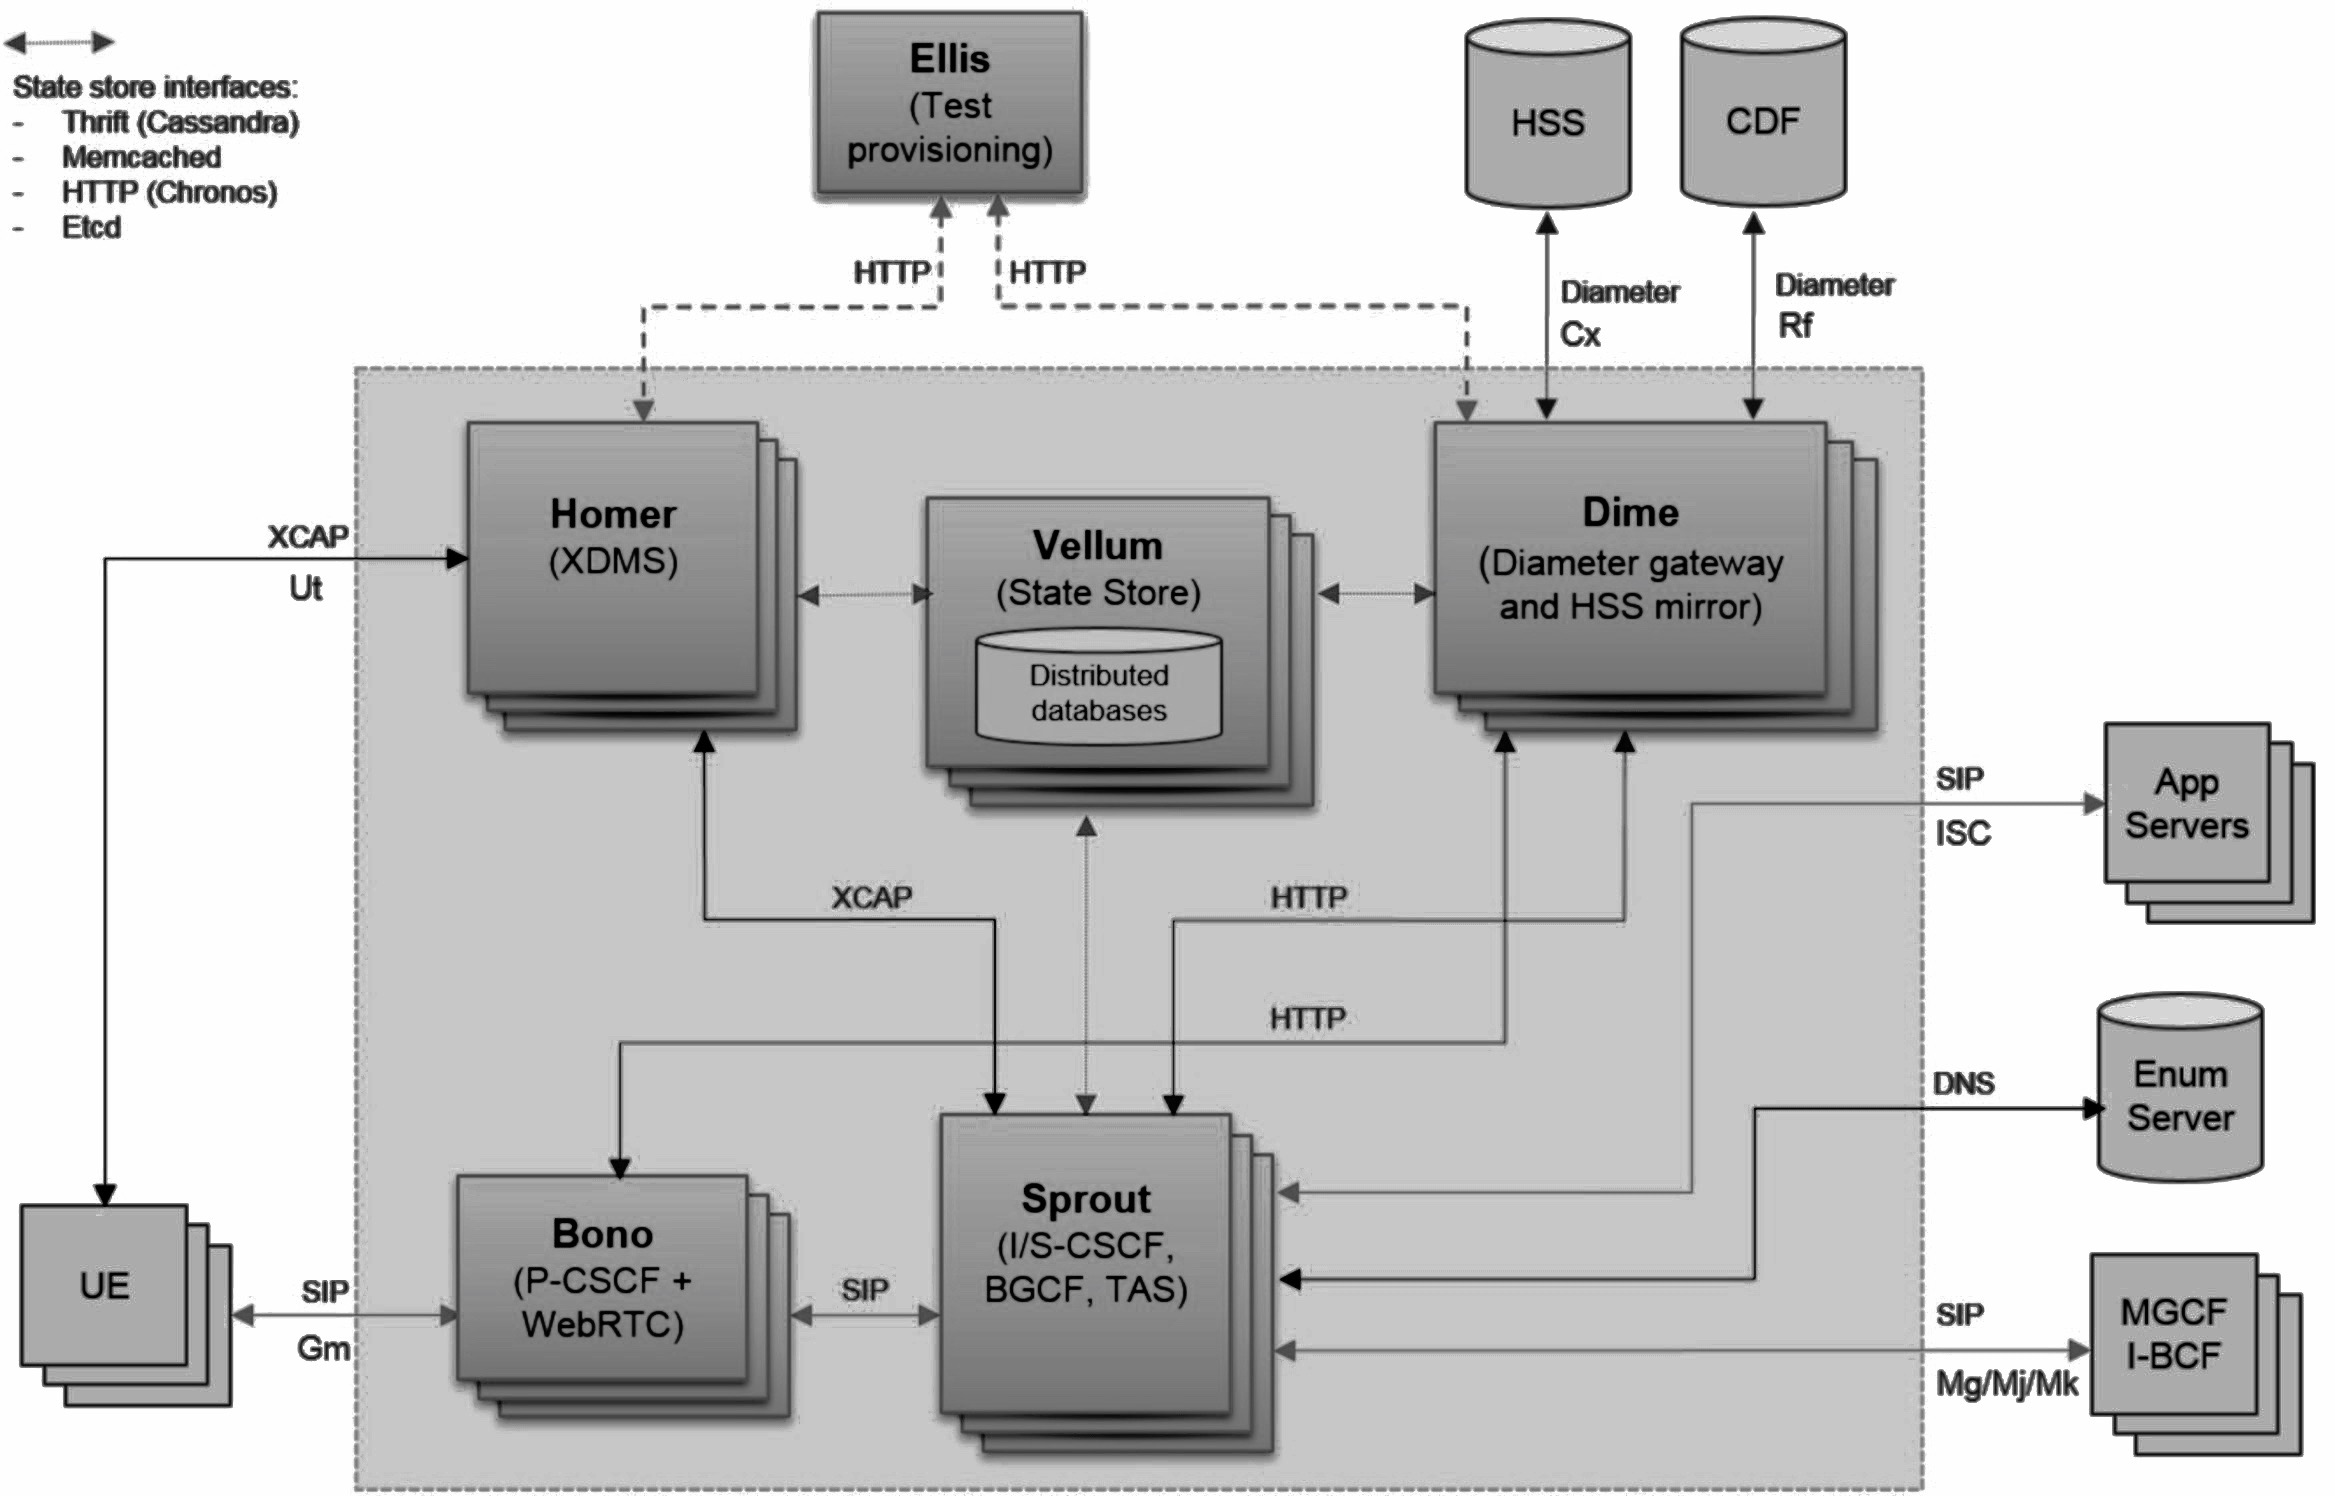
\includegraphics[width=\textwidth]{cwarch}
\caption{معماری \lr{clearwater}}
\label{cwarch}
\end{figure}

\subsubsection{\lr{Bono}}
این المان، نقش \lr{P-CSCF} را دارد و نقطه\nf ی ورود به \lr{IMS} می\nf باشد. فراهم کردن مکانیزم عبور از \lr{NAT}\RTLfootnote{سرواژه\nf ی عبارت \lr{Network Address Translation}} و دیوار آتش\RTLfootnote{\lr{Firewall}} توسّط این المان انجام می\nf شود. کاربران می\nf توانند با استفاده از پیام\nf های \lr{SIP} به \lr{Bono} متّصل شوند؛ این پیام\nf های \lr{SIP} می\nf توانند از پروتکل\nf های لایه\nf ی انتقال \lr{UDP} و \lr{TCP} استفاده کنند.  همچنین، المان \lr{Bono} شامل رابط \lr{webRTC} برای کاربران نیز می\nf باشد و سیگنالینگ\nf های ایجاد تماس را با استفاده از \lr{SIP} بر روی سوکت وب انجام می\nf دهد. \lr{clearwater} می\nf تواند با استفاده از \lr{P-CSCF}های شخص ثالث و یا با استفاده از یک \lr{SBC}\RTLfootnote{سرواژه\nf ی عبارت \lr{Session Border Controller} و به معنای کنترل کننده\nf ی مرز جلسه}که \lr{P-CSCF} را پیاده\nf سازی کرده است، راه\nf اندازی شود؛ در این صورت دیگر نیازی به المان \lr{Bono} نیست.



\subsubsection{\lr{Sprout} (مسیریاب  \lr{SIP})}
المان \lr{Sprout}، به\nf طور هم\nf زمان نقش \lr{I-CSCF, S-CSCF, BGCF} و \lr{TAS} را دارد. این المان، شامل اپلیکیشن سرور \lr{MMTEL}\RTLfootnote{کوتاه\nf شده\nf ی عبارت \lr{Multimedia Telephony}. اپلیکیشن سرور \lr{MMTEL}، به\nf صورت پیش\nf فرض در معماری \lr{clearwater} وجود دارد و با استفاده از آن می\nf توان تماس صوتی یا تصویری و همچنین سرویس پیامک را برقرار کرد .} نیز می\nf باشد. تراکنش\nf های \lr{SIP}، به\nf صورت متوازن در خوشه\nf ی\RTLfootnote{\lr{Cluster}} \lr{Sprout} پخش شده\nf اند. بنابراین هیچ وابستگی طولانی مدّت بین کاربر و یک نود خاص \lr{Sprout} وجود ندارد؛ در نتیجه،  \lr{Sprout} هیچ دیتای طولانی مدّت را ذخیره نمی\nf کند، امّا از طریق رابط سرویس وب، به \lr{Homestead} و \lr{Homer} متّصل شده و اطّلاعات لازم را از \lr{HSS} به\nf دست می\nf آورد. نود \lr{Sprout}، از طریق رابط برنامه\nf نویسی اپلیکیشن، برای ذخیره\nf ی دیتای ثبت\nf نام مشترکین و همچنین راه\nf اندازی زمان\nf سنج، به \lr{Vellum} متّصل می\nf شود. بسیاری از کارکردهای \lr{I-CSCF} و \lr{S-CSCF} در \lr{Sprout} پیاده\nf سازی شده\nf اند و مابقی کارکردها توسّط المان \lr{Dime} تأمین می\nf شوند.

\subsubsection{\lr{Dime} (درگاه \lr{Diameter}) }
\label{dime}
نود \lr{Dime}، دو المان \lr{clearwater} به نام\nf های \lr{Homestead} و \lr{Ralf} را اجرا می\nf کند.
\begin{itemize}
\item \lr{Homestead} (ذخیره\nf گاه \lr{HSS})
\end{itemize}

\indent این المان، رابط سرویس وب را برای \lr{Sprout} فراهم می\nf کند تا \lr{Sprout} بتواند اطّلاعات مربوط به احراز هویّت و اطّلاعات پروفایل کاربران را به\nf دست آورد.

\begin{itemize}
\item \lr{\lr{Ralf}}
\end{itemize}

\indent این المان، یک رابط برنامه\nf نویسی اپلیکشن \lr{HTTP} را برای \lr{Bono} و \lr{Sprout} فراهم می\nf کند. المان\nf های \lr{Sprout} و \lr{Bono}، با استفاده از این رابط گزارش رخدادهای صورت\nf حسابی\RTLfootnote{\lr{Billable}} کاربران را به المان \lr{CDF} ارسال می\nf کنند. المان \lr{Ralf} از المان \lr{Vellum} برای نگه\nf داری اطّلاعات طولانی مدّت وضعیت جلسات استفاده می\nf کند.


\subsubsection{\lr{Vellum} (محل ذخیره\nf ی وضعیت)}
\label{vellum}
المان \lr{Vellum}، تمام وضعیت\nf های طولانی مدّت را نگه\nf می\nf دارد. این کار با اجرای خوشه\nf های حافظه\nf ی توزیع\nf شده به نام \lr{Cassandra} انجام می\nf شود. \lr{Cassandra}، یک پایگاه داده\nf ی متن\nf باز و توزیع\nf شده است که برای مدیریت حجم   زیادی از داده\nf ها در سرورهای مختلف استفاده می\nf شود. توزیع\nf شده بودن این پایگاه داده، در دسترس بودن و قابلیت اطمینان را فراهم می\nf کند\cite{cassandra}.

\subsubsection{\lr{Homer}}

این المان، یک سرور مدیریّت دیتای \lr{XML} است که مستندات مربوط به تنظیمات سرویس \lr{MMTEL} را برای هر کاربر ذخیره می\nf کند. همانند سایر المان\nf ها، \lr{Homer} از نود \lr{Vellum} برای ذخیره\nf ی تمام دیتاهای طولانی مدّت استفاده می\nf کند. 


\subsubsection{\lr{Ellis}}

نود \lr{Ellis}، کارهایی مانند نام\nf نویسی\RTLfootnote{\lr{Sign-up}}، مدیریت رمزعبور، کنترل خط و همچنین کنترل تنظیمات سرویس \lr{MMTEL} را آسان کرده و به\nf صورت خودکار انجام می\nf دهد. این نود ، به\nf عنوان یک المان اصلی پروژه\nf ی \lr{clearwater} شناخته نمی\nf شود؛ بلکه برای راحت کردن استفاده از این پروژه طرّاحی شده است. با توجّه به پیاده\nf سازی \lr{Ellis} با استفاده از \lr{MySQL}، مقیاس کردن آن کاری دشوار و پیچیده است. 


\section{قابلیت های \lr{clearwater}}


 پروژه\nf ی \lr{clearwater}، بسیاری از کاربردهای استاندارد \lr{IMS} را پشتیبانی می\nf کند. از پیاده\nf سازی \lr{clearwater} می\nf توان به عنوان یک سیستم خوداتّکا برای ارائه\nf ی سرویس \lr{VOIP} در بستر شبکه\nf ی محلّی و یا اینترنت استفاده کرد. این سیستم، قابلیت اتّصال به سایر سیستم\nf های ارائه\nf دهنده\nf ی سرویس تماس صوتی نظیر \lr{PSTN}، سایر شبکه\nf های \lr{VOIP} و \lr{webRTC} را دارد. همچنین، می\nf توان با اتّصال \lr{clearwater} به شبکه\nf ی سلولی، سرویس تماس صوتی را از طریق \lr{IP} و با کیفیّت تضمین\nf شده را به مشترکین اپراتورها ارائه کرد.

از دیگر قابلیت\nf های این سیستم، امکان اضافه کردن اپلیکشن سرور است. توسعه\nf دهندگان نرم\nf افزار، می\nf توانند اپلیکیشن سرورهای جدید برای ارائه\nf ی کاربردهای نوظهور طرّاحی کنند و به\nf راحتی این اپلیکیشن سرورها را به معماری \lr{clearwater} اضافه کنند. لذا، ارائه\nf ی سرویس\nf های نوظهور بر مبنای \lr{IMS}، از قابلیت\nf های \lr{clearwater} به\nf شمار می\nf رود. از دیگر قابلیت\nf های این پروژه، عدم وابستگی به ناحیه\nf ی دسترسی است(بخش \ref{benefitsPart}). 

مقیاس\nf پذیری این سیستم، چه در بستر سخت\nf افزاری و چه در بستر ابر، از قابلیت\nf های مهم این سیستم به\nf شمار می\nf رود. \lr{clearwater} به\nf گونه\nf ای طرّاحی شده است که مقیاس کردن آن آسان است. این سیستم، قابلیت ایجاد خوشه\nf ای از نودهای یکسان را دارد. با ایجاد خوشه\nf ای از یک نود، قابلیت اطمینان سیستم و همچنین سرعت و کارایی سیستم افزایش می\nf یابد و سیستم قادر به ارائه\nf ی سرویس به کاربران بیشتری می\nf شود. می\nf توان با ایجاد یک افزونگی جغرافیایی از کل معماری سیستم، پس از به\nf وجود آمدن نقص در سیستم اصلی، همچنان سرویس خود را ارائه کنیم. با ایجاد افزونگی جغرافیایی، در صورت از کار افتادن سیستم اصلی می\nf توان با استفاده از روش\nf های ارائه\nf شده، پیکربندی و داده\nf های موجود در آن را بازیابی کرد.

  

